Um die Entwicklung für die Codebasis so einfach wie möglich zu machen wurde Git verwendet. Es handelt sich um ein Versionskontrollsystem, das hauptsächlich von Entwicklern zur Verwaltung der verschiedenen Versionen ihres Codes verwendet wird. Das Ziel hinter Git steckt darin die Entwicklung für ein Team von mehrern Entwicklern so einfach wie möglich zu gestalten. Im April 2005 begann der Entwickler des Betriebssystems Linux Linus Torvalds mit der Entwicklung von Git und präsentierte bereits wenige Tage nach der Ankündigung die erste Version der Code Verwaltungs Software.

\begin{figure}[h!]
    \centering
    
\includegraphics[width=0.5\linewidth]{pics/git-logo.png}
    \caption{Git Logo}
    \label{fig:enter-label}
\end{figure}

\cite{Git}

\subsubsection{Repository}

Ein Git-Repository ist ein Speicherort, in dem Git, ein weit verbreitetes Versionskontrollsystem, Dateien und Verzeichnisse speichert. Bereits ein normaler Ordner kann ein Repository werden. Hierzu muss nur ein spezieller Befehl im Terminal ausgeführt werden, dieser erstellt einen .git Ordner in welchem die verschiedenen Versionen der Dateien gespeichert werden. Wichtig zu wissen ist auch das die Dateien im .git Ordner nicht manuell geändert werden sollten, da dies zu Problemen führen könnte.

\subsubsection{Commit}

Um eine neue Version von einer oder mehreren Dateien zu speichern muss ein Commit gemacht werden. Bevor ein Commit gemacht wird müssen die einzelnen Änderungen in den sogenannten "Staging-Bereich" hinzugefügt werden. Es können entweder spezifische Dateien hinzugefügt werden oder alle Dateien welche Änderungen beinhalten. Zum Beispiel :

\begin{verbatim}
git add <dateiname>.txt # Eine bestimmte Datei hinzufügen
git add . # Alle geänderten Dateien hinzufügen
\end{verbatim}

\subsubsection{Branches}

Branches werden in größeren Entwickler Teams meistens für einzelne Features verwendet. Somit wird sichergestellt, dass die einzelnen Teammitglieder nicht versehentlich Änderungen in einer Datei vornehmen die für ein anderes Feature essenziell sind. Beim erstellen von einem Branch wird im Hintergrund an und für sich nur eine Kopie des main Branches erstellt. Der Branch kann mit dem Befehl: 

\begin{verbatim}
    git checkout <branchname>
\end{verbatim}

gewechselt werden.
In einem Branch kann der Entwickler quasi frei arbeiten ohne die Arbeit eines Teammitglieds zu bearbeiten, solange er seinen Branch nicht in einen anderen merged.

<image>

\cite{Github_Branches}

\subsubsection{Merge}

Mit dem Merge Befehl werden einer oder mehrere Zweige (Branches) zusammengeführt. Dies ist in Git eine sehr häufige Operation welche verwendet wird um den Code aus einem Quellzweig in den Zielzweig zu bringen.
Ein Merge wird mit folgendem Befehl ausgeführt: 

\begin{verbatim}
    git merge <branchname>
\end{verbatim}

Hierbei kann es zu Konflikten kommen. Dies geschieht normalerweise, wenn zwei oder mehr Zweige gleichzeitig Änderungen an derselben Stelle in einer Datei oder an einer Datei vornehmen. Git kann hier nicht automatisch entscheiden welche Version es behalten soll und so muss der User manuell entsheiden welche Version verwertet und welche verworfen werden soll. Mit dieser Funktion können Änderungen von Zweigen sehr einfach in den Main Branch gebracht werden.

\subsubsection{Submodules}

In der Softwareentwicklung kommt es des öfteren vor, dass während der Entwicklung auch andere Projekte oder Libraries benötigt werden. Häuftig entsteht dabei das Problem, dass beide Projekte seperat behandelt werden müssen. Git behebt diese Problem mit der Hilfe von Submodulen. Diese ermöglichen es ein Projekt als Unterverzeichnis in ein anderes Projekt zu implementieren.

Ein Submodule wird folgendermaßen implementiert:

\begin{lstlisting}
git submodule add https://github.com/chaconinc/DbConnector
\end{lstlisting}

Mit diesem Befehl wird das Subprojekt in ein Unterverzeichnis mit dem Namen des Repositorys in diesem Fall "DbConnector" geschrieben. Dieser Name kann im Nachhinein verändert werden.

Danach wird eine ".gitmodules" Datei erstellet. In dieser kann der Name und der Pfad des Submodules verändert werden.
\begin{lstlisting}
[submodule "DbConnector"]
	path = DbConnector
	url = https://github.com/chaconinc/DbConnector
\end{lstlisting}

Wenn ein Github Repository gecloned wird welches ein Submodule enthält sieht der Konsolen Output folgendermaßen aus. 
\begin{lstlisting}
$ git clone https://github.com/chaconinc/MainProject
Cloning into 'MainProject'...
remote: Counting objects: 14, done.
remote: Compressing objects: 100% (13/13), done.
remote: Total 14 (delta 1), reused 13 (delta 0)
Unpacking objects: 100% (14/14), done.
Checking connectivity... done.
$ cd MainProject
$ ls -la
total 16
drwxr-xr-x   9 schacon  staff  306 Sep 17 15:21 .
drwxr-xr-x   7 schacon  staff  238 Sep 17 15:21 ..
drwxr-xr-x  13 schacon  staff  442 Sep 17 15:21 .git
-rw-r--r--   1 schacon  staff   92 Sep 17 15:21 .gitmodules
drwxr-xr-x   2 schacon  staff   68 Sep 17 15:21 DbConnector
-rw-r--r--   1 schacon  staff  756 Sep 17 15:21 Makefile
drwxr-xr-x   3 schacon  staff  102 Sep 17 15:21 includes
drwxr-xr-x   4 schacon  staff  136 Sep 17 15:21 scripts
drwxr-xr-x   4 schacon  staff  136 Sep 17 15:21 src
$ cd DbConnector/
$ ls
$
\end{lstlisting}

Aktuell ist der DbConnector Ornder noch leer. Um das Submodule zu initialiseren müssen zwei Befehle ausgeführt werden:

\begin{lstlisting}
git submodule init
git submodule update
\end{lstlisting}

In dieser Diplomarbeit wurden Submodules verwendet, da auch parallel immer das Planfred Projekt gestartet sein muss, da die Write-Operationen über die Planfred Datenbank ausgeführt werden. Somit war es anfangs sehr kompliziert, da immer beide Projekte gleichzeitig laufen mussten und dadurch die Ports auch teilweise doppelt belegt wurden, was zu einem Fehler geführt hat.

Um das Planfred Projekt zu initialisieren wurden im 'package.json' folgendes Script geschrieben:

\begin{lstlisting}
"_install:submodule:planfred": "([ -f \"./planfred/package.json\" ] && (cd planfred; npm i;) || echo 'planfred/package.json not found - so no install.')"
\end{lstlisting}

Im ersten Schritt wird überprüft ob im Verzeichnis "planfred" eine Datei mit dem Name "package.json" vorhanden ist. Im nächsten Schritt wird mit "cd planfred" in das Verzeichnis gewechselt und mit "npm i" werden alle nötigen Abhängigkeiten des Projekts (wie in der "package.json"-Datei angegeben) installiert. Falls die "package.json"-Datei nicht gefunden wird, wird der Teil nach || ausgeführt. In diesem Fall wird eine Meldung ausgegeben, die besagt, dass die "package.json"-Datei nicht gefunden wurde und daher keine Installation durchgeführt wurde.




https://git-scm.com/book/en/v2/Git-Tools-Submodules

\begin{figure}[h!]
    \centering
    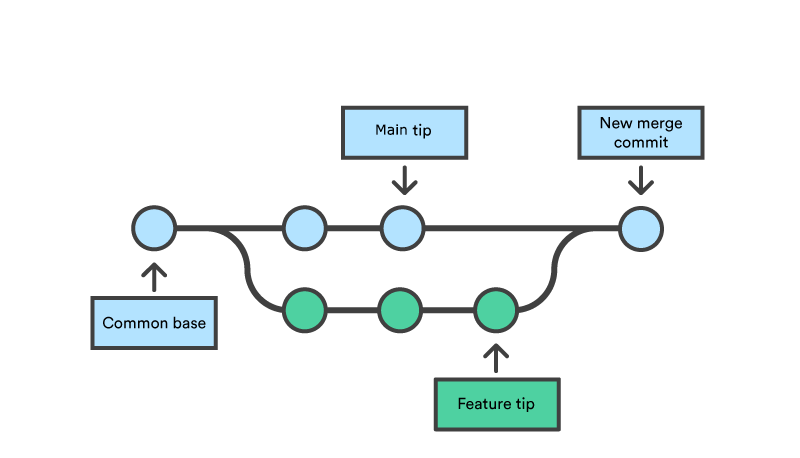
\includegraphics[width=0.6\linewidth]{pics/merge.png}
    \caption{Wie funktioniert ein Merge}
    \label{fig:enter-label}
\end{figure}

\subsection{Git cloud solutions}

Um als Team mit Git zu arbeiten ist es wichtig, dass alle Änderungen zwischen den Usern und den verschiedenen Geräten synchronisiert werden. Hierfür werden Git cloud solutions verwendet. Eine der bekanntesten ist Github, diese Plattform wird von den meisten Entwicklern verwendet.

\subsubsection{Github}

Github ist einer der Gründe wieso Git so berühmt wurde. Es wurde 2008 gelaunched und war damals eine der ersten git hosting Plattformen welche die Zusammenarbeit zwischen mehreren Entwicklerun um einiges vereinfachte. Github bietet sehr viele kostenlose Features an solange das Repository öffenltich ist. Um ein privates Repository zu besitzen und diese Features trotzdem verwenden zu können ist ein Abonnoment nötig.

\cite{Github_1}
\cite{Github_2}